  \documentclass[a4j,twocolumn]{jsarticle}
  \usepackage[dvipdfmx]{graphicx}
  \usepackage{url}

  \setlength{\textheight}{275mm}
  \headheight 5mm
  \topmargin -30mm
  \textwidth 185mm
  \oddsidemargin -15mm
  \evensidemargin -15mm
  \pagestyle{empty}


  \begin{document}

  \title{旅行プランニングアプリの開発}
  \author{情報科学科 \hspace{5mm} 37022463 \hspace{5mm} 山本果音}
  \date{}

  \maketitle


\section{序論}
\label{sec:org6d65ae4}
旅行時に活用される代表的なアプリケーションとして、Google マップ[1]が挙げられる。
Google マップは、ユーザーのニーズに応じて目的地の検索やルートの確認を行うことができる地図サービスであり、個人
の関心に合わせて地図を作成・カスタマイズする機能を備えている[2]。
しかし、Google マップを旅行のプランニングツールとして活用する場合、以下のような課題が存在する。
\begin{enumerate}
\item 複数のスポットを登録すると訪問順序が分かりにくい。
\item 各スポットへの到着時間を地図上に示すことができないため、旅行全体の時間配分や移動の流れが把握しづらくなる。
\end{enumerate}
結果として登録した情報が時系列で整理されず、旅行メンバー間でのプラン共有や調整に混乱が生じ、最終的に使われなくなってしまう。
そこで、各スポットの到着時間を含めた旅行先の情報を分かりやすく整理し、日付やカテゴリごとに参照・共有することを習慣化でき
る旅行プランニングアプリの開発を行う。


\begin{figure}[htbp]
\centering
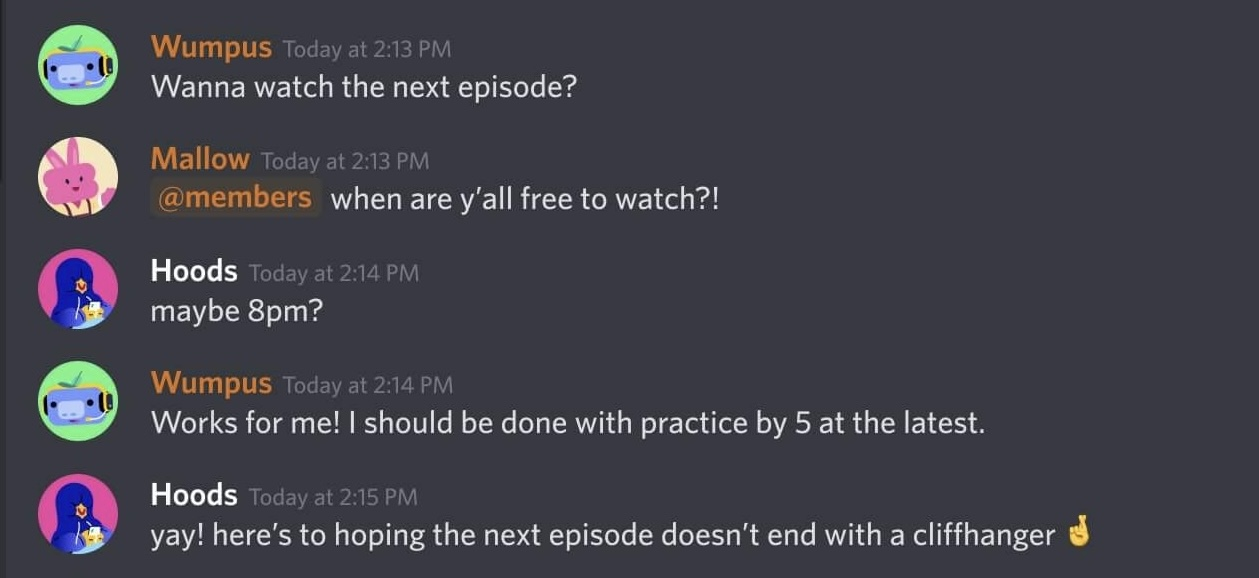
\includegraphics[width=7cm]{./figs/discord.jpg}
\caption{\label{fig:org4bc6090}Googleマップで旅行プランを立てた場合の画面}
\end{figure}


\section{開発手法}
\label{sec:org0bfd248}
Django,python


開発環境としてRuby on Rails(Rails)[3]を選定した.
Railsの利点は以下の4点である.
\begin{enumerate}
\item 広いプラットフォームからのアプリ利用が可能.
\item 日本語のドキュメントが充実しているため開発ハードルが低い[4].
\item ライブラリが豊富.
\item クラウドプラットフォームHeroku[5]との連携が容易.
\end{enumerate}
データの分類方法としては「超」整理法[6]の時間軸をキーとして分類する方式を採用する.
Railsと「超」整理法の時間軸整理を組み合わせ,
データを日付ごとに管理することによって出席状況や,
その日に取ったメモなどを一目で把握できるWebアプリを開発する.



\section{結果}
\label{sec:org2f19e6f}
今回、開発したWebアプリでの情報共有のメリットは以下の2点である.
\begin{enumerate}
\item 投稿されたデータは保存したい日付を1つのカラムに保持しているため、日付ごとのデータ管理が容易.
\item 投稿されたデータ一覧画面では、タグでのデータ絞り込み機能が利用可能.
\end{enumerate}
また,どちらのアプリもログイン済みであることを前提として,投稿されたデータを参照するまでのアクション数を比較する.
Discordではサーバーの選択、チャンネルの選択、画面のスクロールなど最低でも3つのアクションを
要する.
私が開発したWebアプリでは日付選択の1アクションでデータを参照することが可能である.
\begin{figure}[htbp]
\centering
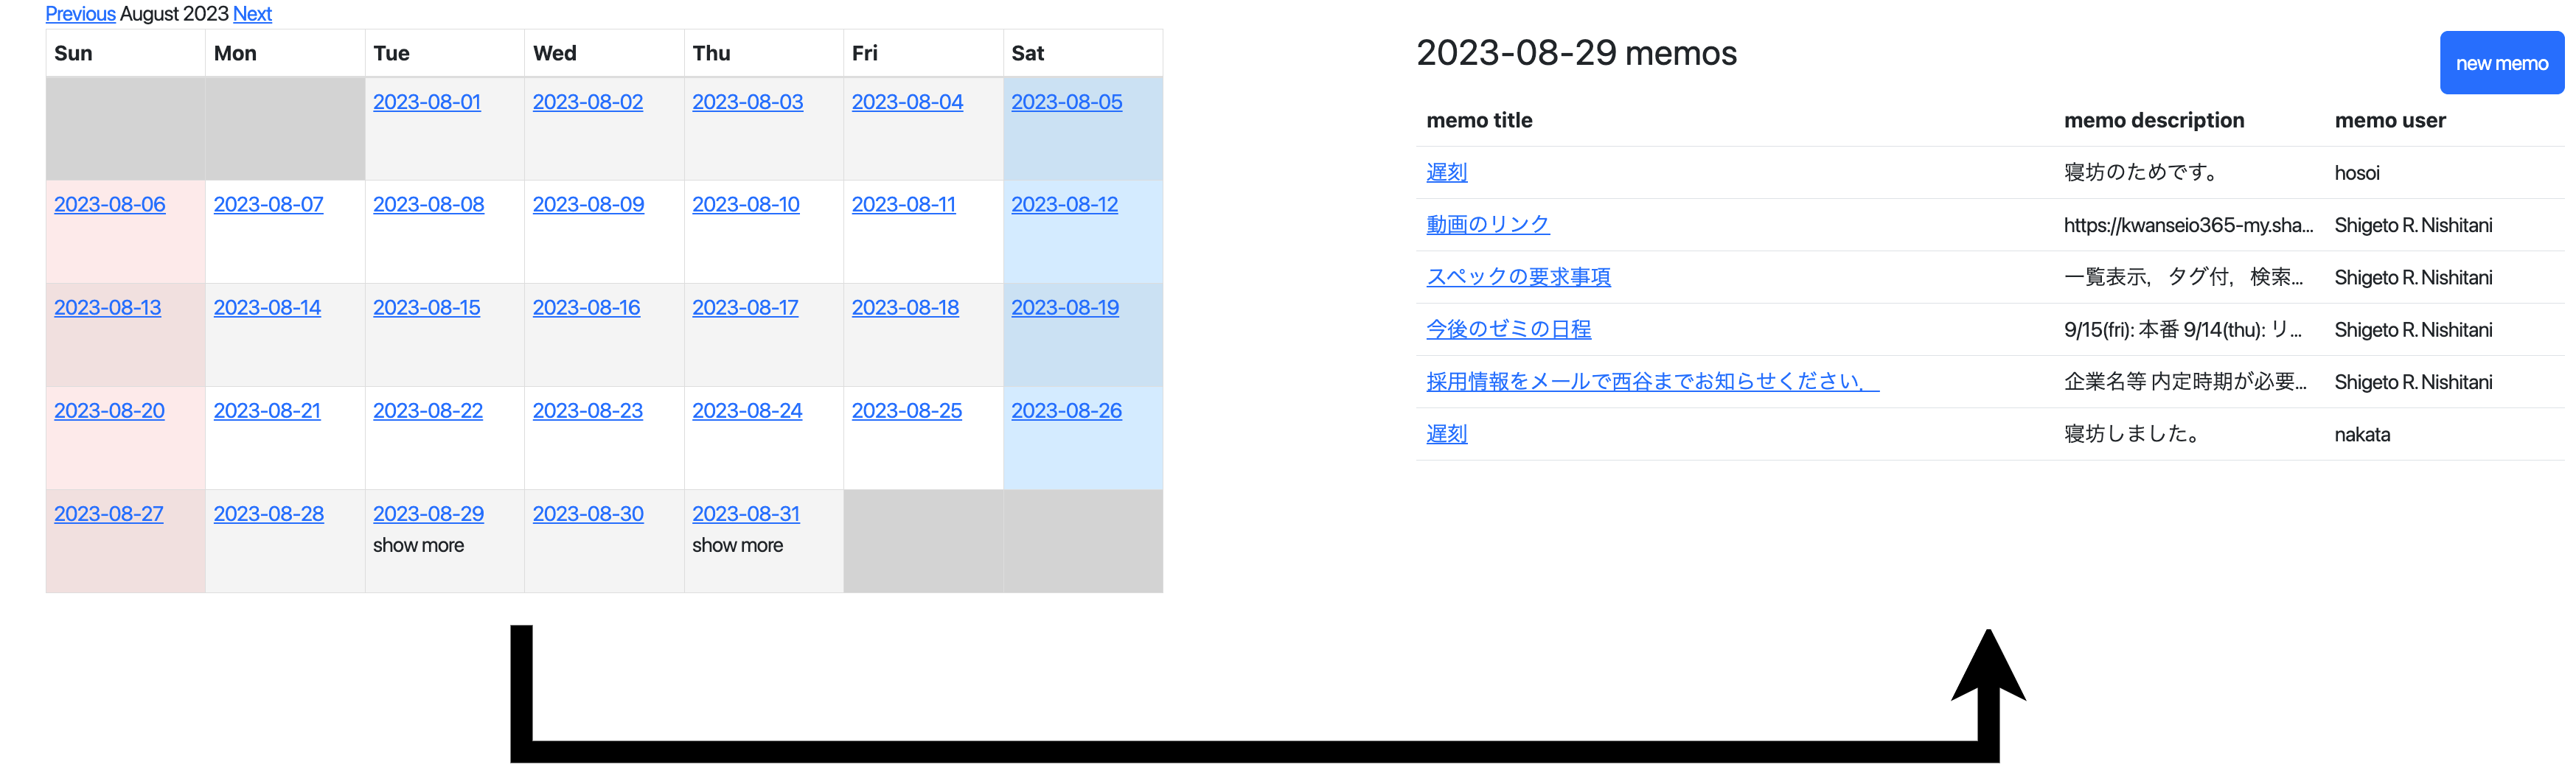
\includegraphics[width=10cm]{./figs/app_motion.png}
\caption{\label{fig:org18cdb57}参照したい日付に保存されたデータを参照する一連の動作.}
\end{figure}


\section{今後の課題}
\label{sec:org463d252}
今回は基本的なCreate(生成),Read(読み取り),Update(更新),Delete(削除)処理(CRUD処理)に加えて,
データの絞り込み機能,グループ作成,メンバー招待・参加機能を開発した.
今後は共有データの見逃しを防ぐための通知機能,ローカルPC上で作成したメモから
このWebアプリへの送信スクリプトを開発する.
また,閲覧回数などの要素から共有データを重みづけし,不要なデータは自動的に削除する機能も組み込み,
更なる共有データの整理,Webアプリのパフォーマンス向上を図る.


\small\setlength\baselineskip{10pt}
\begin{thebibliography}{9}
\bibitem{Discord Inc.}Discord, https://www.google.co.jp/intl/ja/maps/about/mymaps/.
\bibitem{Discord background} Discord会社概要, https://discord.com/company.
\bibitem{Copyright (c) YassLab 株式会社} Ruby on Railsチュートリアル, https://railstutorial.jp.
\bibitem{Railsドキュメント (c) 2023} Ruby on Railsドキュメント(v7.0.0), https://railsdoc.com.
\bibitem{Heroku} WHAT IS HEROKU?, https://www.heroku.com/what.
\bibitem{noguchi} 野口 悠紀雄, 「超」整理法―情報検索と発想の新システム (中公新書), 中央公論新社, (1993).
\end{thebibliography}
\end{document}
